\chapter{Experimental Dataset}
This chapter describes the dataset and the experimental procedure used in this research for developing machine learning applications. First, the cyclic fatigue testing was conducted till the fracture of a material to acquire the fatigue characteristics of a material. Second, to mimic the scenarios in the remanufacturing industry, interrupted fatigue testing was utilized to produce specimens at different fatigue levels as a representation of end-of-life products. Linear and nonlinear ultrasound measurements are used to evaluate the fatigue damage of those specimens stopped at the predetermined number of cycles in the interrupted fatigue test. Besides, the residual stress and full width at half maximum data from X-ray diffraction are also presented.

\section{Life cycle fatigue testing}
The life cycle fatigue testing aims to collect the fatigue life data to understand the fatigue behavior of our targeted material. The fatigue life of a material is defined as the total number of cycles that a material can sustain under a specified loading condition. In order to develop the S-N curve of a material, the material is tested at different loading stress amplitudes, and the fatigue test is repeated multiple times for each loading stress amplitude to account for the variance of fatigue life.

The fatigue testing in this research is led by Prof. Li's group at the Penn State University. The targeted material is 5052-H32 aluminum alloy which is widely used for car body construction in the automotive industry. Figure \ref{fig: fatigue testing setup} shows the dimension of the specimen and the test machine. Three loading amplitudes, 11.7, 12.7, and 14.7 kN for the cyclic fatigue testing are selected to develop the S-N curve which is shown in Figure \ref{fig: raw sn curve}. 

\begin{figure}[tb]
  \begin{subfigure}[t]{0.50\linewidth}
    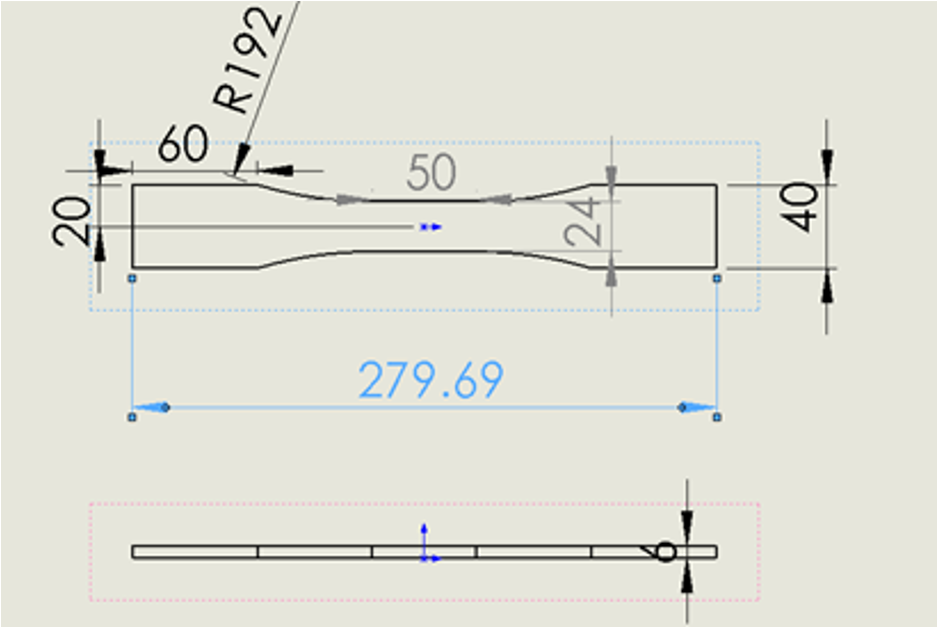
\includegraphics[height=0.7\textwidth]{fig/specimen_dim.png}
    \caption{Schematic of the 5052-H32 aluminum alloy specimen}
    \label{fig: specimen dim}
  \end{subfigure}
  \begin{subfigure}[t]{0.50\linewidth}
    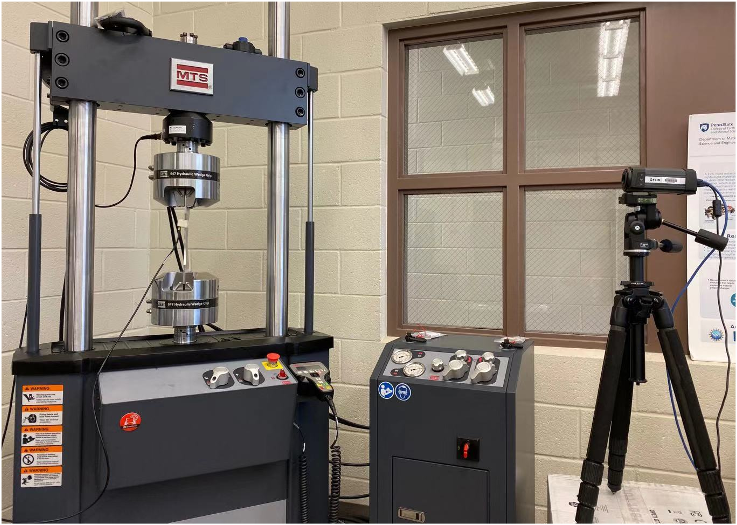
\includegraphics[height=0.7\textwidth]{fig/fatigue_testing_machine.png}
    \caption{MTS 100KN Landmark fatigue testing system at Prof. Jingjing li's lab}
    \label{fig: fatigue testing machine}
  \end{subfigure}

  \caption{Life cycle fatigue testing setup}
  \label{fig: fatigue testing setup}
\end{figure}

\begin{figure}[tb]
  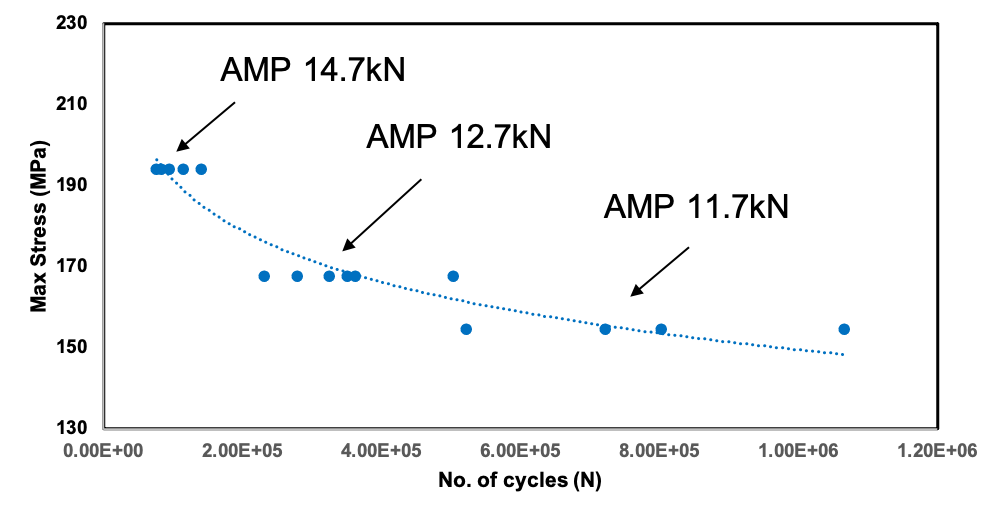
\includegraphics[width=\linewidth]{fig/sn_curve.png}
  \caption{S-N curve for 5052-H32 aluminum alloy}
  \label{fig: raw sn curve}
\end{figure}

\section{Interrupted fatigue testing}
The purpose of performing interrupted fatigue testing is to produce specimens at various fatigue levels by stopping the testing at several predetermined number of cycles. Considering the material cost and the time spent, the number of cycles applied to the specimens is set to be two levels, 33\% and 67\% fatigue life corresponding to the three loading amplitudes, 11.7, 12.7, and 14.7 kN. These specimens are used to represent the end-of-life products having different fatigue damage levels in the remanufacturing industry. Besides, three specimens without going through fatigue testing, i.e., 0\% fatigue life, are included as specimens at the healthy state. The summary of the interrupted fatigue testing specimens is presented in Table \ref{table: interrupted specimens}

\begin{table}[tb]
  \centering
  \caption{Summary of the interrupted fatigue testing specimens}
  \label{table: interrupted specimens}
  \begin{tabularx}{\textwidth}{
    >{\centering\arraybackslash}X|
    >{\centering\arraybackslash}X|
    >{\centering\arraybackslash}X|
    >{\centering\arraybackslash}X
  }\hline\hline
    Specimen ID&Loading Amplitude (kN)&Percentage of Fatigue Life (\%)&Max Stress Applied (MPa)\\\hline
    1&11.7&33&176\\
    2&11.7&33&176\\
    3&11.7&67&176\\
    4&11.7&67&176\\
    5&12.7&33&195\\
    6&12.7&33&195\\
    7&12.7&67&195\\
    8&12.7&67&195\\
    9&14.7&33&221\\
    10&14.7&33&221\\
    11&14.7&67&221\\
    12&14.7&67&221\\
    13&--&0&--\\
    14&--&0&--\\
    15&--&0&--\\\hline
  \end{tabularx}
\end{table}

\section{Linear and nonlinear ultrasound measurements}
Linear ultrasonic (LU) and nonlinear ultrasonic (NLU) testing serve as the two main NDE methods for measuring the accumulated fatigue damage in the specimens. The ultrasonic testing is led by Prof. Matlack's group, and the ultrasound testing system is shown in Figure \ref{fig: ultrasound setup}. The LU and NLU measurements are both 1-D time domain signals, but the two approaches differ based on the different theories and parameters, e.g., excitation wave shape, frequency, amplitude, etc. Examples of LU and NLU signals are presented in Figure \ref{fig: lu and nlu signals raw}.

LU and NLU measurements were collected at nine locations in a specimen as illustrated in Figure \ref{fig: measurement locations}, and each location was measured three times to ensure the measurement repeatability. As a result, for each specimen, there are $9 \times 3 = 27$ signal profiles produced.

\begin{figure}[tb]
  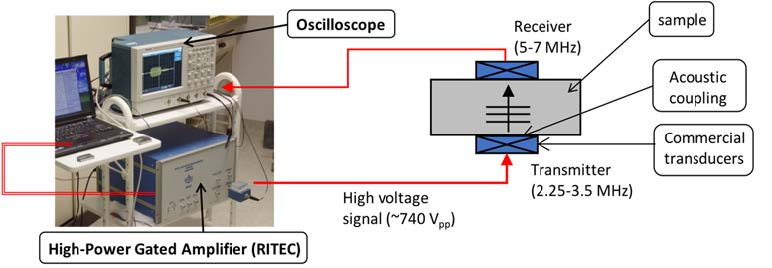
\includegraphics[width=\linewidth]{fig/ultrasound setup.png}
  \caption{Experimental setup for LU and NLU at Prof. Matlack's Lab}
  \label{fig: ultrasound setup}
\end{figure}

\begin{figure}[tb]
  \begin{subfigure}[t]{0.50\linewidth}
    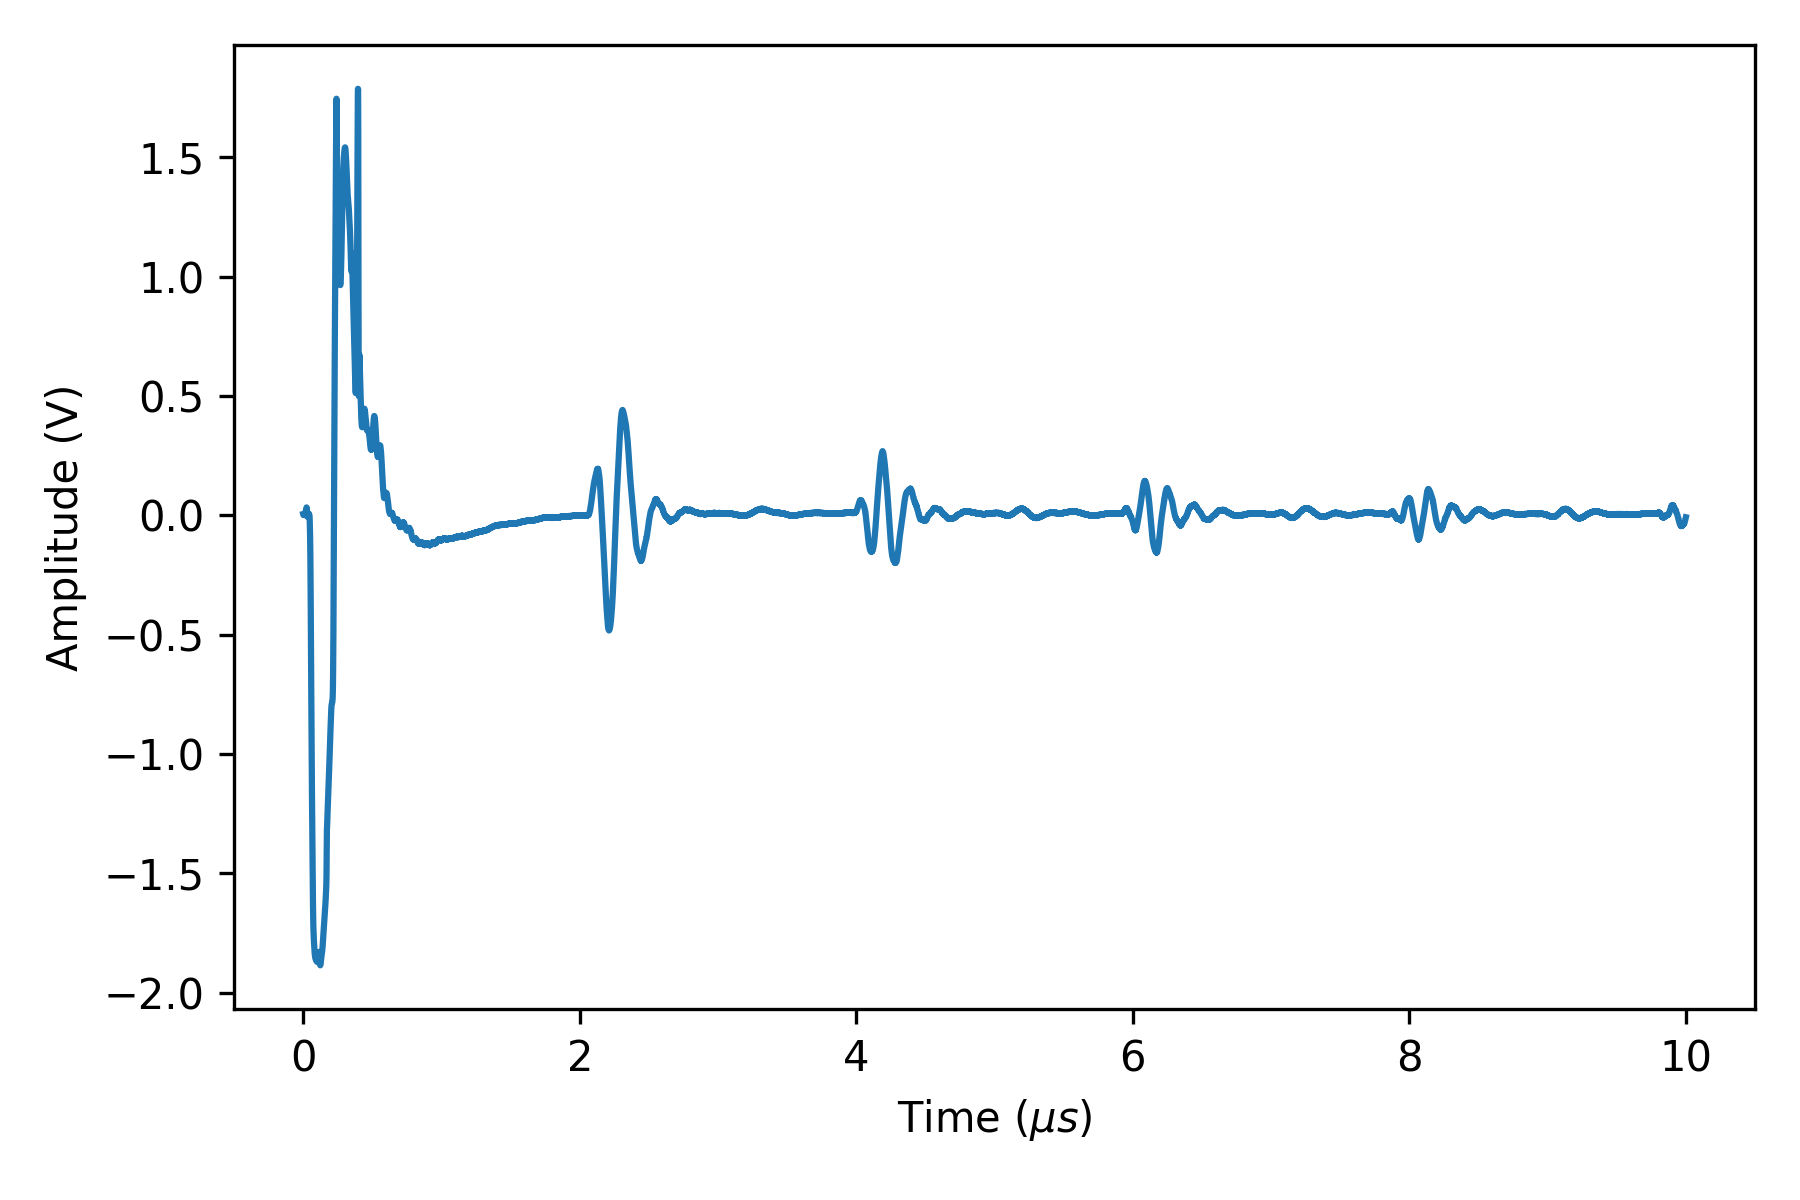
\includegraphics[width=\textwidth]{fig/lu_signal_raw.png}
    \caption{Linear ultrasonic signal}
    \label{fig: lu signal raw}
  \end{subfigure}
  \begin{subfigure}[t]{0.50\linewidth}
    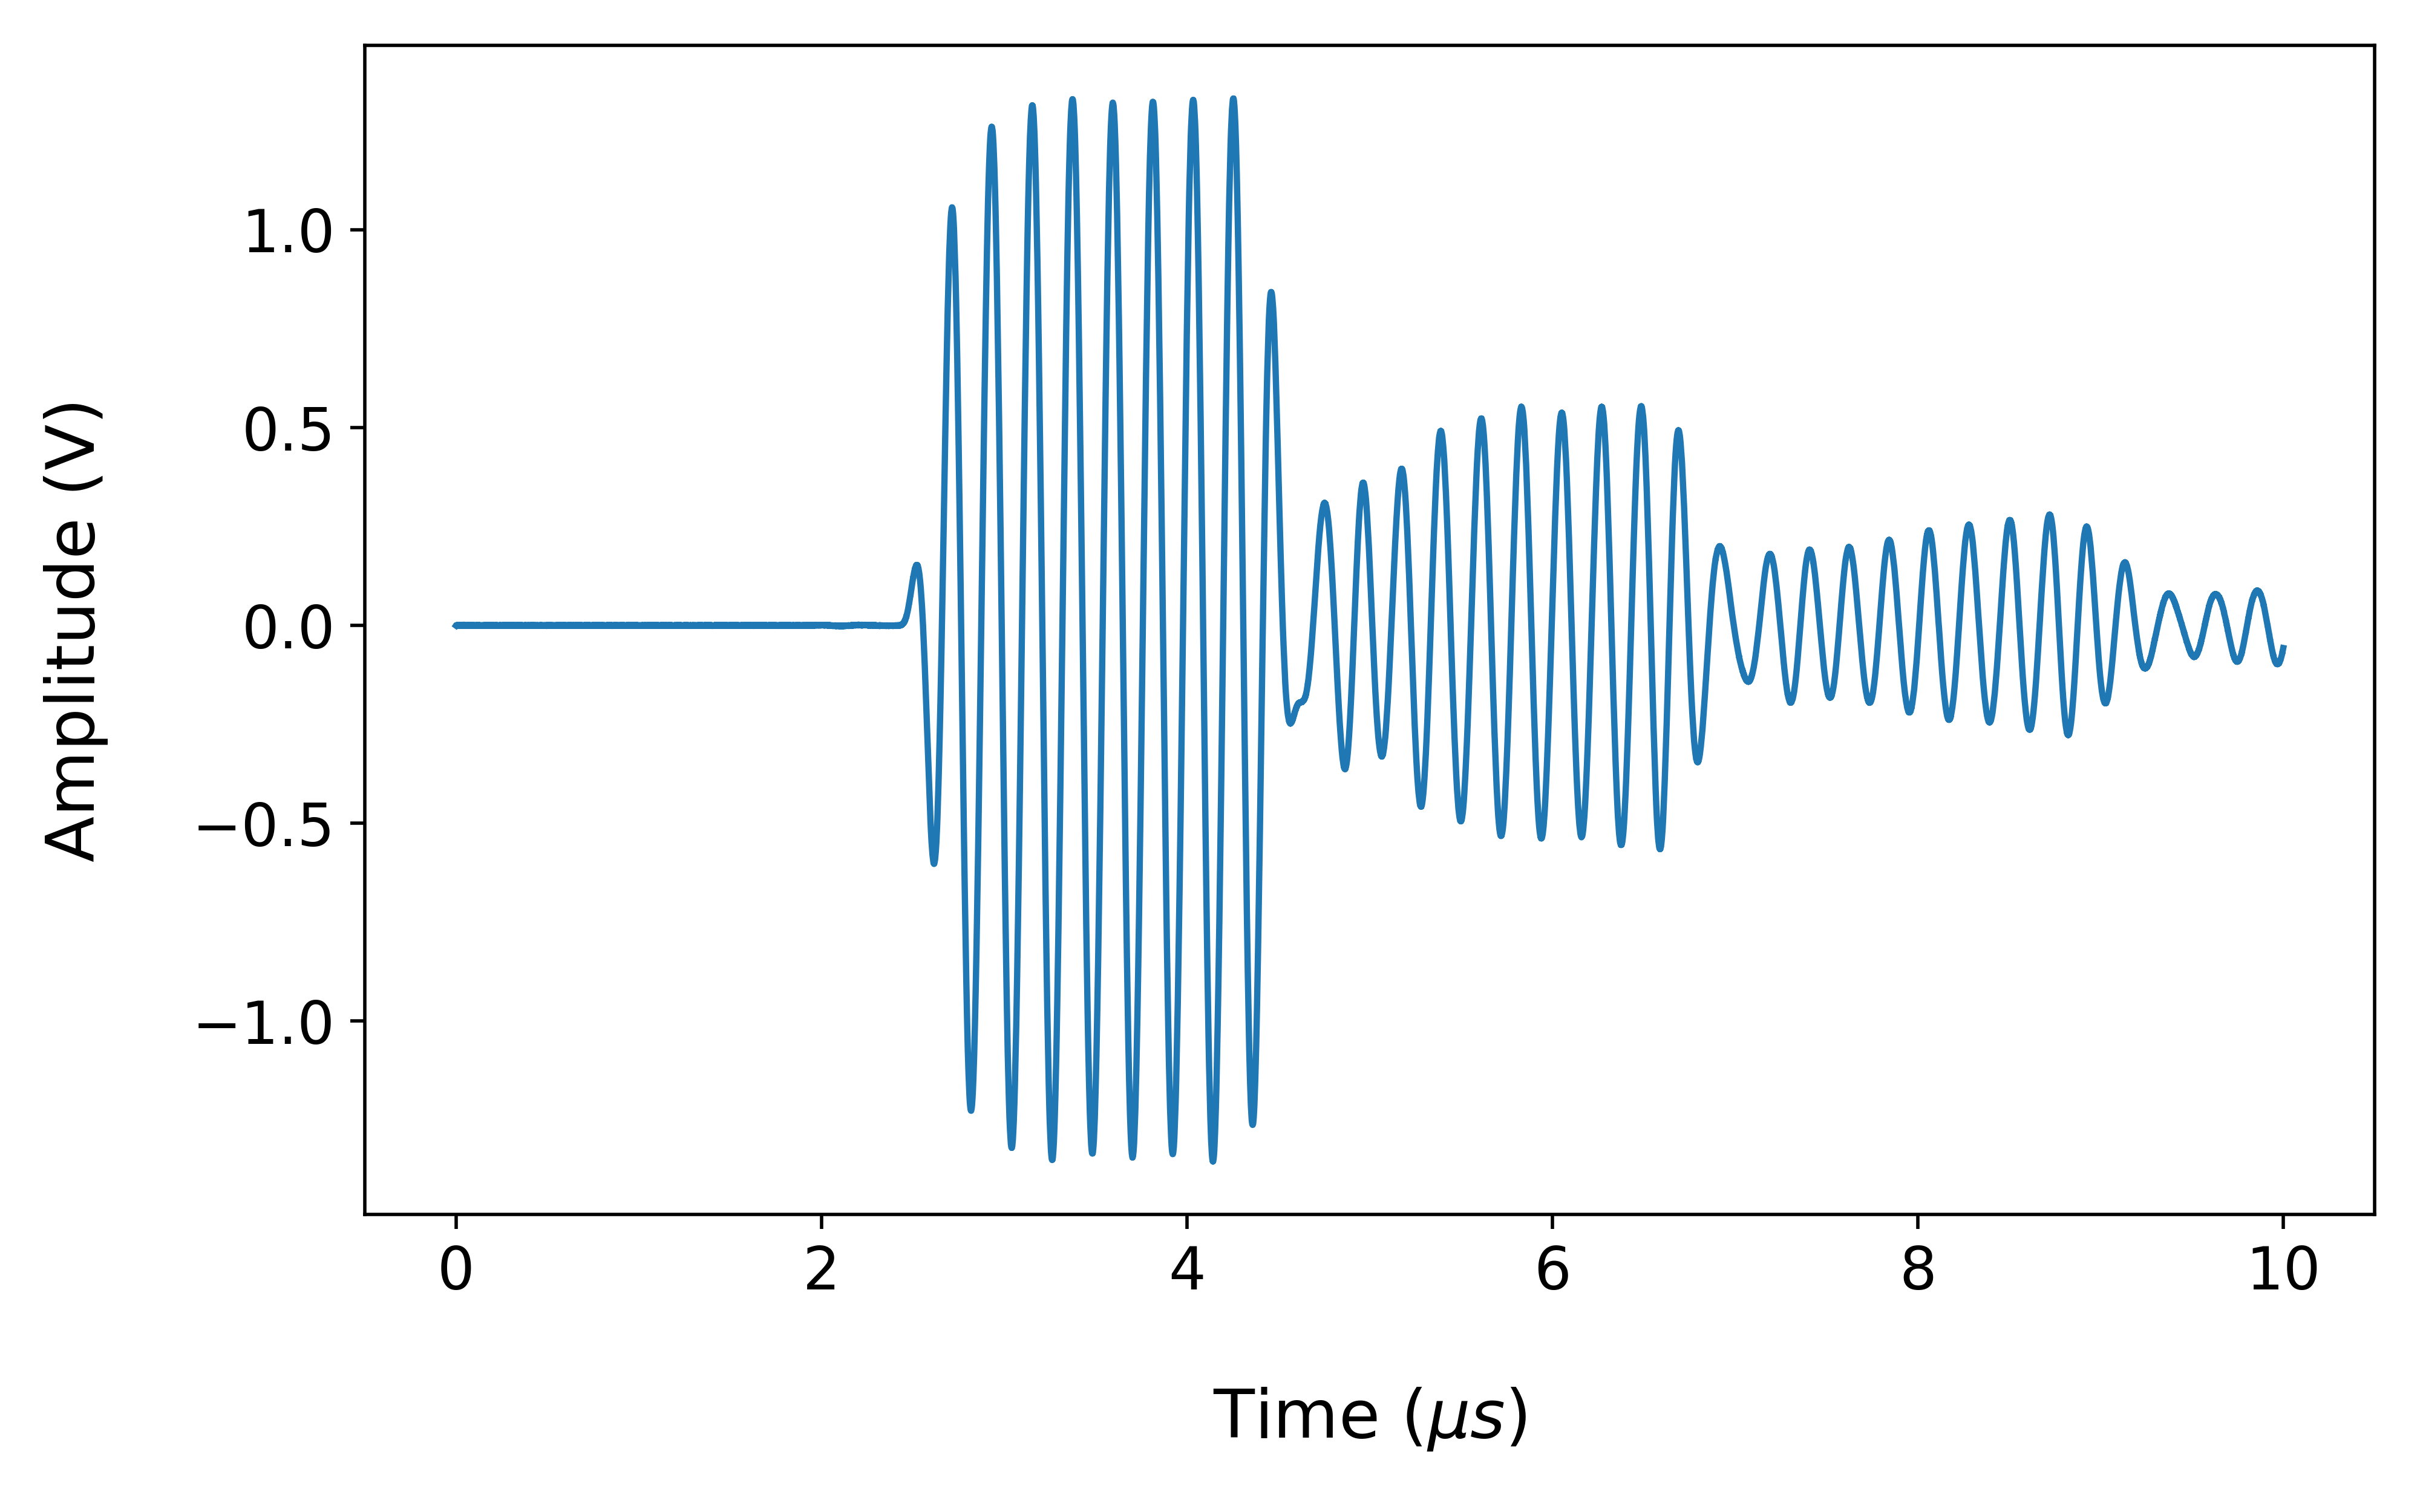
\includegraphics[width=\textwidth]{fig/nlu_singal_raw.png}
    \caption{Nonlinear ultrasonic signal}
    \label{fig: nlu signal raw}
  \end{subfigure}

  \caption{Examples of linear and nonlinear ultrasonic signals}
  \label{fig: lu and nlu signals raw}
\end{figure}

\begin{figure}[tb]
  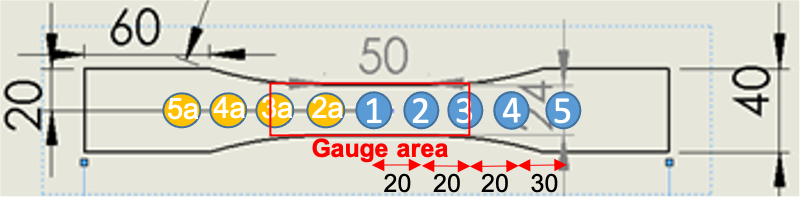
\includegraphics[width=\linewidth]{fig/specimen_measurment_locs.png}
  \caption{Schematic of the measurement locations for LU and NLU measurements. (The unit of length is in mm)}
  \label{fig: measurement locations}
\end{figure}

\section{X-ray diffraction measurement}
Another quantity of interest, residual stress, is measured by X-ray diffraction (XRD) in this research. Residual stress is known to be associated with fatigue behaviors such as crack initiation and propagation. Besides, the full width at half maximum height (FWHM) of the diffraction peak in XRD is also calculated. Prof. Li's group performed the XRD measurements for a subset of specimens in the interrupted fatigue testing specimens. The XRD data is used in the regression tasks in Chapter.
